\section{证据依赖、威胁传播与动态推理}
\subsection{带类型的对象依赖图}

令 $G_t=(V_t,E_t)$ 为一个以时间为索引的有向多重图，其节点是 OAL 对象及其版本或状态区间。关系明确其语义：实体\emph{控制}平台；平台\emph{承载}模型或\emph{产生}观测；路径\emph{传输}产品；实体对产品\emph{背书}或\emph{使用}产品；记录对另一产品\emph{作出承诺}。一次转换将其输入、输出、执行平台、责任实体、代码/模型版本和事件区间连接起来。在 PROV 中，该转换可以序列化为活动\citep{w3c2013provdm}。图~\ref{fig:dependency} 展示这些依赖及其证据状态。

\begin{figure}[!htbp]\centering
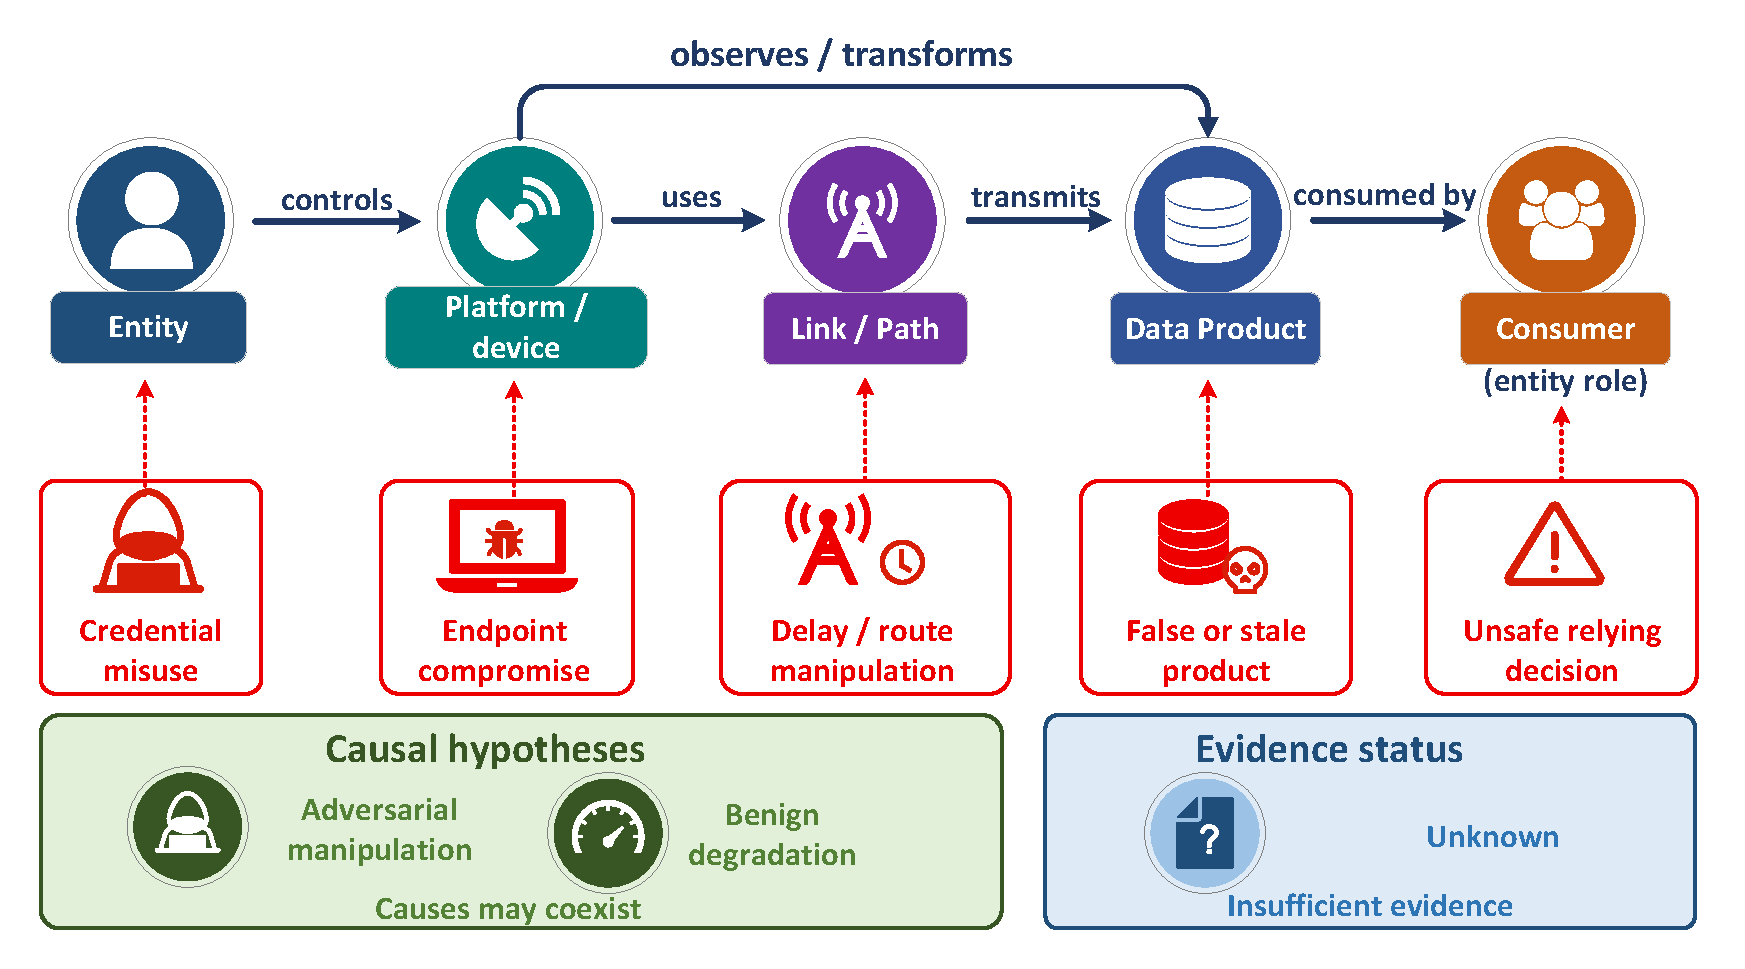
\includegraphics[width=\textwidth]{figures/figure-04-dependency-threat.pdf}
\caption{带类型的依赖与证据状态。运行关系识别假设变化所影响的主张。非恶意退化和对抗性干预属于因果假设；未知属于认识层面的结果。}\label{fig:dependency}
\end{figure}

当密钥、端点、模型或输入发生争议时，通过图遍历识别需要重新评估的主张。仅有一条图边，不能量化因果影响，也不足以支持概率更新。交叉佐证必须考虑共享的数据源、时钟、转换过程和管理根源。从同一观测派生的两个产品，并不构成两次独立观测。反之，共享中继不一定会使其他方面独立的数据源的端到端签名失效。

\subsection{威胁、退化与证据缺失}

分析陈述应识别攻击者或环境原因及其相关能力，再沿受影响对象和传播关系追踪至任务后果。同时记录控制措施和剩余不确定性。例如，被攻陷的 USV 可以扣留 UUV 批次，延迟使用者获得证据和开展审计；独立接触机会与受保护的本地计数器，可能在重连后暴露缺口。声学衰落也可能造成相同的交付症状，但原因不同。在原因归属仍未知时，可以限制对时效性敏感的用途。表~\ref{tab:threats} 汇总部分跨对象故障路径。

\begin{table}[H]\small
\caption{所选故障路径的跨对象分析。}\label{tab:threats}
\begin{tabularx}{\textwidth}{LLL}\toprule
\textbf{初始条件} & \textbf{受影响的依赖} & \textbf{证据与响应}\\\midrule
凭证被盗 & 从实体权限到签名产品 & 按生效时间撤销；审查签名的派生后代\\
端点被攻陷 & 从设备状态到观测或转换 & 证明范围、诊断与交叉佐证；隔离受影响输出\\
衰落或干扰 & 从路径可用性到证据时效性 & 信道/情境证据；限制过时信息的使用，保留原因不确定性\\
相关数据源 & 从共享输入到融合结论 & 谱系与共同原因模型；减少独立证据计数\\
治理法定人数不可用 & 从共享策略到新的全局权限 & 保留先前检查点；执行有界本地委托\\\bottomrule
\end{tabularx}\end{table}

\subsection{CTG 推理循环}

CTG 通过图~\ref{fig:ctg} 中的八步循环，利用情境、时间状态和依赖关系指导评估及策略行动。证据捕获包括绑定验证；依赖传播识别受影响的派生后代，以便在明确的推断规则下重新评估。

MAPE-K 提供监控、分析、规划、执行和共享知识\citep{kephart2003autonomic,ibm2005mapek}。CTG 将这些功能应用于主张评估，区分事件时间和接收时间，并通过已记录的依赖关系触发重新评估。JDL 融合模型区分对象、态势、影响和过程优化\citep{steinberg1999jdl}。针对这些估计，CTG 记录依赖决策所需的身份、溯源、治理和时间证据。

实现可以采用贝叶斯模型、主观逻辑、隐状态推断、规则或学习型分类器。输出保留所指属性、情境、证据谱系、不确定性和允许用途。变化后重新估计信任，需要明确的更新规则，而不是沿图边任意扣减。硬性授权条件可以与分级质量估计共存；是否将某项条件设为不可由其他指标补偿，由任务策略决定。

\begin{figure}[!htbp]\centering
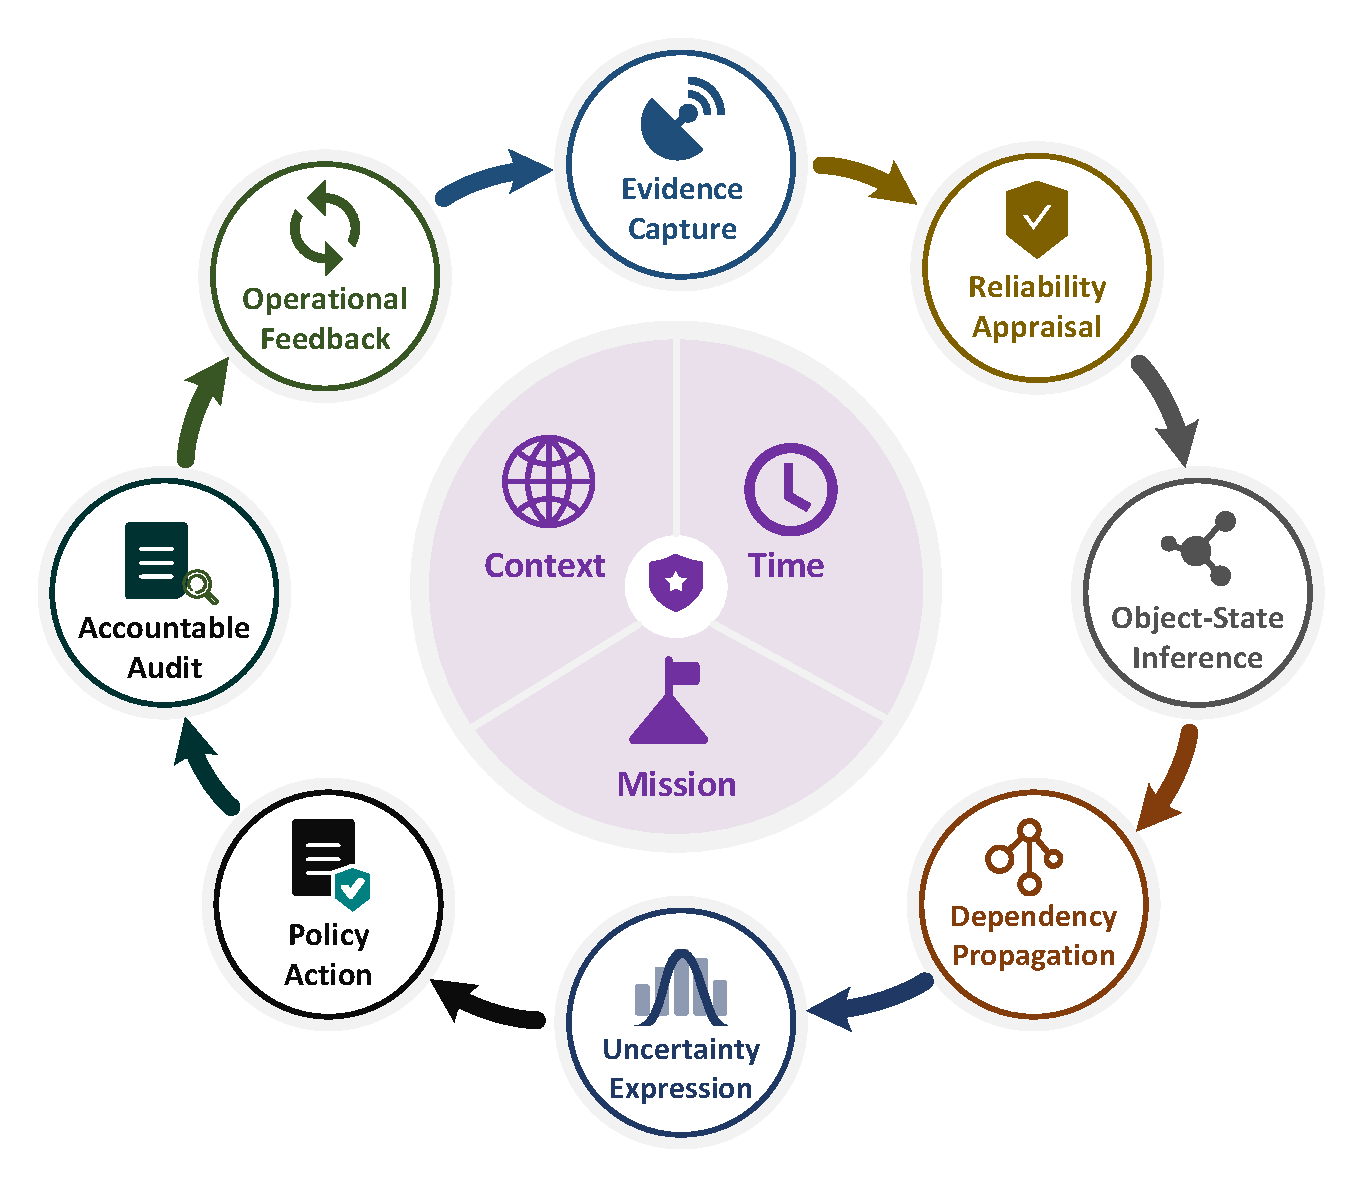
\includegraphics[width=.78\textwidth]{figures/figure-05-ctg-reasoning-loop.pdf}
\caption{CTG 评估与行动循环，各步骤共享策略、时间状态和依赖知识。}\label{fig:ctg}
\end{figure}

\subsection{分区、撤销与协调轨迹}\label{sec:trace}

第~\ref{sec:coalition} 节的联盟已共同批准策略版本 1，以及一项在 $t=480$ s 到期、适用于低后果用途的本地委托。在 $t=0$ 时，USV 失去岸端连接；在 $t=240$ s 时，岸端组织提交对一个 UUV 签名密钥的撤销，立即生效。UUV 在 $t=600$ s 重连时收到撤销信息。其受保护时钟报告事件区间，而不是精确事件时间。该场景假定保留事件具有可信的、被攻陷之前的时间/计数器记录；仅凭被盗密钥无法建立可信的历史时间戳。

三条签名记录的区间分别为 $[114,126]$、$[234,246]$ 和 $[294,306]$ s。重连后，验证方检查源签名、批次包含关系、策略纪元和撤销历史。区间在 240 s 之前结束的记录，可以具备历史审计资格；区间在 240 s 或之后开始的记录，在事件时刻已被撤销；跨越 240 s 的区间被隔离，等待复核。具备历史资格，不会授权新的物理行动，也不会使观测重新变得新鲜。

示例均值对签名有效性、观测质量、谱系、缓存策略匹配和时间权限取平均，使用 $[1,0.95,1,1,a]$，其中 $a=1,0.5,0$，阈值为 0.75。这种可补偿聚合接受全部三条记录。加入明确权限否决条件的标量策略，则产生与带类型规则完全相同的决策。决策差异源于策略是否将时间权限作为否决条件执行。表~\ref{tab:trace} 报告回放结果。

\begin{table}[H]\small
\caption{可执行回放结果。账本与具有策略验证能力的见证日志路径使用相同的证据和授权规则。标量示例使用相同的输入特征。}\label{tab:trace}
\begin{tabularx}{\textwidth}{@{}P{25mm}YP{21mm}Y@{}}\toprule
\textbf{事件区间（s）} & \textbf{OAL 组织的规则/验证日志} & \textbf{均值分数} & \textbf{标量决策}\\\midrule
114--126 & 合格的历史记录 & 0.99 & 均值接受；带否决条件的标量与规则一致\\
234--246 & 隔离：与撤销时点重叠 & 0.89 & 均值接受；带否决条件的标量将其隔离\\
294--306 & 在事件时刻已撤销 & 0.79 & 均值接受；带否决条件的标量拒绝\\\bottomrule
\end{tabularx}\end{table}

断连期间，420 s 时的行动可在缓存运行边界内获得受限本地权限，即使后续审计发现其与已生效的全局撤销相冲突；到 540 s 时，该边界已到期，本地策略拒绝行动。协调过程同时保留当时本地可用的权限与后续全局判断。若改写旧决策，仿佛航行器在 240 s 时就收到了撤销信息，就会抹去这一区别。

合成回放验证 Ed25519 签名与 Merkle 包含关系，拒绝遭修改的记录/证明，检查带重复交付的全部六种到达顺序，并枚举联盟签名者的全部 16 个子集。账本策略与验证日志的决策函数在所有情况下均一致。第~\ref{sec:pattern} 节说明相同的应用规则如何映射到 Fabric，以及资源受限航行器如何接收可审计结果。
